\documentclass{beamer}

\mode<presentation> {

%\usetheme{default}
%\usetheme{AnnArbor}
%\usetheme{Antibes}
%\usetheme{Bergen}
%\usetheme{Berkeley}
%\usetheme{Berlin}
%\usetheme{Boadilla}
\usetheme{CambridgeUS}
%\usetheme{Copenhagen}
%\usetheme{Darmstadt}
%\usetheme{Dresden}
%\usetheme{Frankfurt}
%\usetheme{Goettingen}
%\usetheme{Hannover}
%\usetheme{Ilmenau}
%\usetheme{JuanLesPins}
%\usetheme{Luebeck}
%\usetheme{Madrid}
%\usetheme{Malmoe}
%\usetheme{Marburg}
%\usetheme{Montpellier}
%\usetheme{PaloAlto}
%\usetheme{Pittsburgh}
%\usetheme{Rochester}
%\usetheme{Singapore}
%\usetheme{Szeged}
%\usetheme{Warsaw}

%\usecolortheme{albatross}
\usecolortheme{beaver}
%\usecolortheme{beetle}
%\usecolortheme{crane}
%\usecolortheme{dolphin}
%\usecolortheme{dove}
%\usecolortheme{fly}
%\usecolortheme{lily}
%\usecolortheme{orchid}
%\usecolortheme{rose}
%\usecolortheme{seagull}
%\usecolortheme{seahorse}
%\usecolortheme{whale}
%\usecolortheme{wolverine}

%\setbeamertemplate{footline} % To remove the footer line in all slides uncomment this line
%\setbeamertemplate{footline}[page number] % To replace the footer line in all slides with a simple slide count uncomment this line
%\setbeamertemplate{navigation symbols}{} % To remove the navigation symbols from the bottom of all slides uncomment this line
}

\usepackage{graphicx}
\usepackage{booktabs}
\usepackage{tikz}
\usepackage{scalefnt}
\usepackage{listings}
\usepackage{todonotes}
\usepackage{tabularx}
\usepackage{enumitem}
\usepackage{hyperref}
\usepackage{xcolor}

\setitemize{label=\usebeamerfont*{itemize item}
\usebeamercolor[fg]{itemize item}
\usebeamertemplate{itemize item}}

\definecolor{ao(english)}{rgb}{0.0, 0.5, 0.0}
\definecolor{aureolin}{rgb}{0.99, 0.93, 0.0}
\definecolor{bostonuniversityred}{rgb}{0.8, 0.0, 0.0}

\renewcommand{\tabularxcolumn}[1]{>{\small}m{#1}}
\renewcommand{\arraystretch}{2}

%% Listings definition for Go language
%% Go language reference : http://www.golang.org
%% Author : Uriel Corfa <uriel@corfa.fr>
%% Project home: https://bitbucket.org/korfuri/golang-latex-listings

\lstdefinelanguage{go}{
  % Keywords as defined in the BNF
  morekeywords=[1]{break,default,func,interface,%
    case,defer,go,map,struct,chan,else,goto,package,%
    switch,const,fallthrough,if,range,type,continue,%
    for,import,return,var,select},
  % Special identifiers, builtin functions
  morekeywords=[2]{make,new,nil,len,cap,copy,complex,%
    real,imag,panic,recover,print,println,iota,close,%
    closed,_,true,false,append,delete},
  % Basic types
  morekeywords=[3]{%
    string,int,uint,uintptr,double,float,byte,%
    int8,int16,int32,int64,int128,%
    uint8,uint16,uint32,uint64,uint128,%
    float32,float64,complex64,complex128,%
    rune},
  % Strings : "toto", 'toto', `toto`
  morestring=[b]{"},
  morestring=[b]{'},
  morestring=[b]{`},
  % Comments : /* comment */ and // comment
  comment=[l]{//},
  morecomment=[s]{/*}{*/},
  % Options
  sensitive=true
}

\lstset{
  language={go},
  basicstyle=\ttfamily\tiny
}

\title[ICS Honeypot]{\textbf{Industrial Control Systems Honeypot}}

\author{May1601}
\institute[]
{
Aashwatth Agarwal \\
Dan Borgerding \\
Jon Hope \\
Nik Kinkel \\
Jon Osborne \\
Korbin Stich \\
\medskip
\url{http://may1601.sd.ece.iastate.edu}\medskip

\textbf{Client}: Alliant Energy

\textbf{Advisor}: Dr. Doug Jacobson
}
\date{\today}

\begin{document}

\begin{titlepage}

\begin{center}

\textup{\small {\bf CPRE/EE/SE 491} \\ Senior Design}\\[0.2in]

% Title
\Large \textbf {May1601 Project Plan}\\[0.5in]

% Submitted by
\normalsize Submitted by \\
\begin{table}[h]
\centering
\begin{tabular}{lr}\hline \\
Jonathan Osborne & Team Leader \\
Nik Kinkel & Key Concept Holder \\ 
Korbin Stich & Key Concept Holder \\ 
Daniel Borgerding & Communication Leader \\ 
Jonathan Hope & Webmaster \\
\\ \hline
%Korbin Stich &  \\ \\ \hline 

\end{tabular}
\end{table}

\vspace{.3in}
Under the guidance of\\
{\textbf{Dr. Doug Jacobson}}\\[0.3in]

\vspace{.3in}
Prepared for\\
{\textbf{Alliant Energy}}\\[0.3in]

\vfill

% Bottom of the page
\vspace{0.2cm}
Fall 2015

\end{center}
\end{titlepage}

\begin{titlepage}
\begin{center}

\vspace*{\fill}
\Huge \textbf {Industrial Control System Honeypot and Traffic Monitor}\\[0.5in]
\vspace*{\fill}

\end{center}
\end{titlepage}

% Slide 1
\begin{frame}
\frametitle{Threat Overview}

\begin{columns}
\column{.4\textwidth}
\vspace{-15mm}
\begin{itemize}
    \item Highly critical threat
    \item Advanced attackers
    \item First attack on a power grid (Ukraine)
\end{itemize}

\column{.6\textwidth}
\begin{figure}[b]
\frame{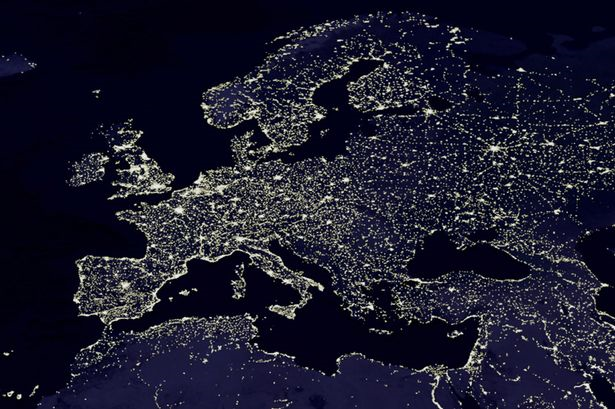
\includegraphics[width=.6\linewidth]{figures/blackout.png}}
\end{figure}
\end{columns}
\end{frame}

% Slide 2
\begin{frame}
\frametitle{Project Overview}

\begin{block}{What is a honeypot?}
A security mechanism desinged to detects, deflects or counteracts attempts at unauthorized use of information systems.
\end{block}
 


\begin{block}{What is the overall goal of the project?}
The goal of the project is to create a standalone security device that can be placed in an industrial network to monitor traffic, looking for security-related irregularities, and act as a low interaction honeypot.
\end{block}
\end{frame}

% Slide 3
\begin{frame}
\frametitle{The Deliverable}

\begin{columns}
\column{.4\textwidth}
\begin{itemize}
    \item Customized honeypots for multiple protocols
    \item Minimal IDS
    \item Automated deployment \& management
    \item Configurable logging backends
    \item Cheap, plug \& play device
\end{itemize}
\column{.6\textwidth}
\begin{figure}[pi]
\frame{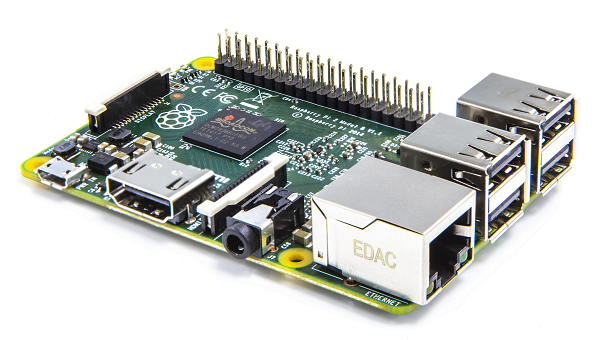
\includegraphics[width=.6\linewidth]{figures/raspi.png}}
\caption*{Raspberry Pi 2}
\end{figure}
\end{columns}
\end{frame}

% Slide 4
\begin{frame}
\frametitle{Risks}

\begin{columns}[c]

\column{0.5\textwidth}
\begin{table}
\begin{center}
\begin{tabular}{l l}
\textbf{Risk} & \textbf{Severity} \\
\midrule
Honeypot exploitation & Critical \\
Infrequent maintenance & High \\
Device fragility & Medium \\
Limited hardware options & Low \\
\bottomrule
\end{tabular}
\end{center}
\end{table}

\column{0.5\textwidth}

TODO: image of network perimeter w/ honeypot inside

\end{columns}

\end{frame}

% Slide 5
\begin{frame}
\frametitle{Tech Challenge 1: Dealing with Lots of Protocols}


\begin{columns}[c]

\column{0.5\textwidth}
4 big problems:

\begin{itemize}
    \item Many different honeypot protocols
    \item New protocols must be integrated quickly
    \item Different logging endpoints
    \item System must be easily extensible
\end{itemize}

\column{0.5\textwidth}

TODO: image showing multiple hpot protos, commin internal repr, then
      multiplexed out to diff logging backends

\end{columns}

\end{frame}

% Slide 6
\begin{frame}
\frametitle{Design: Honeypot Plugin Framework}

\begin{figure}
\centering
\caption{Multi-process, message-passing architecture}
{%\scalefont{0.75}
\scalebox{0.53}{% Graphic for TeX using PGF
% Title: /home/nskinkel/src/may1601/docs/spring2016/final-presentation/dia/hpot-arch.dia
% Creator: Dia v0.97.3
% CreationDate: Thu Apr  7 01:55:27 2016
% For: nskinkel
% \usepackage{tikz}
% The following commands are not supported in PSTricks at present
% We define them conditionally, so when they are implemented,
% this pgf file will use them.
\ifx\du\undefined
  \newlength{\du}
\fi
\setlength{\du}{15\unitlength}
\begin{tikzpicture}
\pgftransformxscale{1.000000}
\pgftransformyscale{-1.000000}
\definecolor{dialinecolor}{rgb}{0.000000, 0.000000, 0.000000}
\pgfsetstrokecolor{dialinecolor}
\definecolor{dialinecolor}{rgb}{1.000000, 1.000000, 1.000000}
\pgfsetfillcolor{dialinecolor}
\pgfsetlinewidth{0.100000\du}
\pgfsetdash{}{0pt}
\pgfsetdash{}{0pt}
\pgfsetmiterjoin
\definecolor{dialinecolor}{rgb}{1.000000, 1.000000, 1.000000}
\pgfsetfillcolor{dialinecolor}
\fill (5.000000\du,5.000000\du)--(5.000000\du,7.000000\du)--(9.000000\du,7.000000\du)--(9.000000\du,5.000000\du)--cycle;
\definecolor{dialinecolor}{rgb}{0.000000, 0.000000, 0.000000}
\pgfsetstrokecolor{dialinecolor}
\draw (5.000000\du,5.000000\du)--(5.000000\du,7.000000\du)--(9.000000\du,7.000000\du)--(9.000000\du,5.000000\du)--cycle;
\pgfsetlinewidth{0.100000\du}
\pgfsetdash{}{0pt}
\pgfsetdash{}{0pt}
\pgfsetmiterjoin
\definecolor{dialinecolor}{rgb}{1.000000, 1.000000, 1.000000}
\pgfsetfillcolor{dialinecolor}
\fill (5.000000\du,8.000000\du)--(5.000000\du,10.000000\du)--(9.000000\du,10.000000\du)--(9.000000\du,8.000000\du)--cycle;
\definecolor{dialinecolor}{rgb}{0.000000, 0.000000, 0.000000}
\pgfsetstrokecolor{dialinecolor}
\draw (5.000000\du,8.000000\du)--(5.000000\du,10.000000\du)--(9.000000\du,10.000000\du)--(9.000000\du,8.000000\du)--cycle;
\pgfsetlinewidth{0.100000\du}
\pgfsetdash{}{0pt}
\pgfsetdash{}{0pt}
\pgfsetmiterjoin
\definecolor{dialinecolor}{rgb}{1.000000, 1.000000, 1.000000}
\pgfsetfillcolor{dialinecolor}
\fill (5.000000\du,11.000000\du)--(5.000000\du,13.000000\du)--(9.000000\du,13.000000\du)--(9.000000\du,11.000000\du)--cycle;
\definecolor{dialinecolor}{rgb}{0.000000, 0.000000, 0.000000}
\pgfsetstrokecolor{dialinecolor}
\draw (5.000000\du,11.000000\du)--(5.000000\du,13.000000\du)--(9.000000\du,13.000000\du)--(9.000000\du,11.000000\du)--cycle;
\pgfsetlinewidth{0.100000\du}
\pgfsetdash{}{0pt}
\pgfsetdash{}{0pt}
\pgfsetmiterjoin
\definecolor{dialinecolor}{rgb}{1.000000, 1.000000, 1.000000}
\pgfsetfillcolor{dialinecolor}
\fill (5.000000\du,19.000000\du)--(5.000000\du,21.000000\du)--(9.000000\du,21.000000\du)--(9.000000\du,19.000000\du)--cycle;
\definecolor{dialinecolor}{rgb}{0.000000, 0.000000, 0.000000}
\pgfsetstrokecolor{dialinecolor}
\draw (5.000000\du,19.000000\du)--(5.000000\du,21.000000\du)--(9.000000\du,21.000000\du)--(9.000000\du,19.000000\du)--cycle;
\pgfsetlinewidth{0.100000\du}
\pgfsetdash{}{0pt}
\pgfsetdash{}{0pt}
\pgfsetmiterjoin
\definecolor{dialinecolor}{rgb}{1.000000, 1.000000, 1.000000}
\pgfsetfillcolor{dialinecolor}
\fill (15.000000\du,9.000000\du)--(15.000000\du,17.000000\du)--(22.000000\du,17.000000\du)--(22.000000\du,9.000000\du)--cycle;
\definecolor{dialinecolor}{rgb}{0.000000, 0.000000, 0.000000}
\pgfsetstrokecolor{dialinecolor}
\draw (15.000000\du,9.000000\du)--(15.000000\du,17.000000\du)--(22.000000\du,17.000000\du)--(22.000000\du,9.000000\du)--cycle;
\pgfsetlinewidth{0.100000\du}
\pgfsetdash{}{0pt}
\pgfsetdash{}{0pt}
\pgfsetmiterjoin
\definecolor{dialinecolor}{rgb}{1.000000, 1.000000, 1.000000}
\pgfsetfillcolor{dialinecolor}
\fill (28.000000\du,5.000000\du)--(28.000000\du,7.000000\du)--(32.000000\du,7.000000\du)--(32.000000\du,5.000000\du)--cycle;
\definecolor{dialinecolor}{rgb}{0.000000, 0.000000, 0.000000}
\pgfsetstrokecolor{dialinecolor}
\draw (28.000000\du,5.000000\du)--(28.000000\du,7.000000\du)--(32.000000\du,7.000000\du)--(32.000000\du,5.000000\du)--cycle;
\pgfsetlinewidth{0.100000\du}
\pgfsetdash{}{0pt}
\pgfsetdash{}{0pt}
\pgfsetmiterjoin
\definecolor{dialinecolor}{rgb}{1.000000, 1.000000, 1.000000}
\pgfsetfillcolor{dialinecolor}
\fill (28.000000\du,8.000000\du)--(28.000000\du,10.000000\du)--(32.000000\du,10.000000\du)--(32.000000\du,8.000000\du)--cycle;
\definecolor{dialinecolor}{rgb}{0.000000, 0.000000, 0.000000}
\pgfsetstrokecolor{dialinecolor}
\draw (28.000000\du,8.000000\du)--(28.000000\du,10.000000\du)--(32.000000\du,10.000000\du)--(32.000000\du,8.000000\du)--cycle;
\pgfsetlinewidth{0.100000\du}
\pgfsetdash{}{0pt}
\pgfsetdash{}{0pt}
\pgfsetmiterjoin
\definecolor{dialinecolor}{rgb}{1.000000, 1.000000, 1.000000}
\pgfsetfillcolor{dialinecolor}
\fill (28.000000\du,11.000000\du)--(28.000000\du,13.000000\du)--(32.000000\du,13.000000\du)--(32.000000\du,11.000000\du)--cycle;
\definecolor{dialinecolor}{rgb}{0.000000, 0.000000, 0.000000}
\pgfsetstrokecolor{dialinecolor}
\draw (28.000000\du,11.000000\du)--(28.000000\du,13.000000\du)--(32.000000\du,13.000000\du)--(32.000000\du,11.000000\du)--cycle;
\pgfsetlinewidth{0.100000\du}
\pgfsetdash{}{0pt}
\pgfsetdash{}{0pt}
\pgfsetmiterjoin
\definecolor{dialinecolor}{rgb}{1.000000, 1.000000, 1.000000}
\pgfsetfillcolor{dialinecolor}
\fill (28.000000\du,19.000000\du)--(28.000000\du,21.000000\du)--(32.000000\du,21.000000\du)--(32.000000\du,19.000000\du)--cycle;
\definecolor{dialinecolor}{rgb}{0.000000, 0.000000, 0.000000}
\pgfsetstrokecolor{dialinecolor}
\draw (28.000000\du,19.000000\du)--(28.000000\du,21.000000\du)--(32.000000\du,21.000000\du)--(32.000000\du,19.000000\du)--cycle;
\pgfsetlinewidth{0.100000\du}
\pgfsetdash{}{0pt}
\pgfsetdash{}{0pt}
\pgfsetbuttcap
{
\definecolor{dialinecolor}{rgb}{0.000000, 0.000000, 0.000000}
\pgfsetfillcolor{dialinecolor}
% was here!!!
\pgfsetarrowsend{latex}
\definecolor{dialinecolor}{rgb}{0.000000, 0.000000, 0.000000}
\pgfsetstrokecolor{dialinecolor}
\draw (9.000000\du,6.000000\du)--(14.950256\du,10.384399\du);
}
\pgfsetlinewidth{0.100000\du}
\pgfsetdash{}{0pt}
\pgfsetdash{}{0pt}
\pgfsetbuttcap
{
\definecolor{dialinecolor}{rgb}{0.000000, 0.000000, 0.000000}
\pgfsetfillcolor{dialinecolor}
% was here!!!
\pgfsetarrowsend{latex}
\definecolor{dialinecolor}{rgb}{0.000000, 0.000000, 0.000000}
\pgfsetstrokecolor{dialinecolor}
\draw (9.000000\du,9.000000\du)--(14.950256\du,11.505371\du);
}
\pgfsetlinewidth{0.100000\du}
\pgfsetdash{}{0pt}
\pgfsetdash{}{0pt}
\pgfsetbuttcap
{
\definecolor{dialinecolor}{rgb}{0.000000, 0.000000, 0.000000}
\pgfsetfillcolor{dialinecolor}
% was here!!!
\pgfsetarrowsend{latex}
\definecolor{dialinecolor}{rgb}{0.000000, 0.000000, 0.000000}
\pgfsetstrokecolor{dialinecolor}
\draw (9.000000\du,12.000000\du)--(15.000000\du,13.000000\du);
}
\pgfsetlinewidth{0.100000\du}
\pgfsetdash{}{0pt}
\pgfsetdash{}{0pt}
\pgfsetbuttcap
{
\definecolor{dialinecolor}{rgb}{0.000000, 0.000000, 0.000000}
\pgfsetfillcolor{dialinecolor}
% was here!!!
\pgfsetarrowsend{latex}
\definecolor{dialinecolor}{rgb}{0.000000, 0.000000, 0.000000}
\pgfsetstrokecolor{dialinecolor}
\draw (9.000000\du,20.000000\du)--(14.950256\du,14.615601\du);
}
\pgfsetlinewidth{0.100000\du}
\pgfsetdash{}{0pt}
\pgfsetdash{}{0pt}
\pgfsetbuttcap
{
\definecolor{dialinecolor}{rgb}{0.000000, 0.000000, 0.000000}
\pgfsetfillcolor{dialinecolor}
% was here!!!
\pgfsetarrowsend{latex}
\definecolor{dialinecolor}{rgb}{0.000000, 0.000000, 0.000000}
\pgfsetstrokecolor{dialinecolor}
\draw (22.049744\du,10.384399\du)--(28.000000\du,6.000000\du);
}
\pgfsetlinewidth{0.100000\du}
\pgfsetdash{}{0pt}
\pgfsetdash{}{0pt}
\pgfsetbuttcap
{
\definecolor{dialinecolor}{rgb}{0.000000, 0.000000, 0.000000}
\pgfsetfillcolor{dialinecolor}
% was here!!!
\pgfsetarrowsend{latex}
\definecolor{dialinecolor}{rgb}{0.000000, 0.000000, 0.000000}
\pgfsetstrokecolor{dialinecolor}
\draw (22.049744\du,11.505371\du)--(28.000000\du,9.000000\du);
}
\pgfsetlinewidth{0.100000\du}
\pgfsetdash{}{0pt}
\pgfsetdash{}{0pt}
\pgfsetbuttcap
{
\definecolor{dialinecolor}{rgb}{0.000000, 0.000000, 0.000000}
\pgfsetfillcolor{dialinecolor}
% was here!!!
\pgfsetarrowsend{latex}
\definecolor{dialinecolor}{rgb}{0.000000, 0.000000, 0.000000}
\pgfsetstrokecolor{dialinecolor}
\draw (22.049744\du,12.626343\du)--(28.000000\du,12.000000\du);
}
\pgfsetlinewidth{0.100000\du}
\pgfsetdash{}{0pt}
\pgfsetdash{}{0pt}
\pgfsetbuttcap
{
\definecolor{dialinecolor}{rgb}{0.000000, 0.000000, 0.000000}
\pgfsetfillcolor{dialinecolor}
% was here!!!
\pgfsetarrowsend{latex}
\definecolor{dialinecolor}{rgb}{0.000000, 0.000000, 0.000000}
\pgfsetstrokecolor{dialinecolor}
\draw (22.049744\du,15.615601\du)--(28.000000\du,20.000000\du);
}
% setfont left to latex
\definecolor{dialinecolor}{rgb}{0.000000, 0.000000, 0.000000}
\pgfsetstrokecolor{dialinecolor}
\node[anchor=west] at (5.900000\du,6.050000\du){SSH};
% setfont left to latex
\definecolor{dialinecolor}{rgb}{0.000000, 0.000000, 0.000000}
\pgfsetstrokecolor{dialinecolor}
\node[anchor=west] at (5.800000\du,9.050000\du){HTTP};
% setfont left to latex
\definecolor{dialinecolor}{rgb}{0.000000, 0.000000, 0.000000}
\pgfsetstrokecolor{dialinecolor}
\node[anchor=west] at (5.600000\du,12.000000\du){HTTPS};
% setfont left to latex
\definecolor{dialinecolor}{rgb}{0.000000, 0.000000, 0.000000}
\pgfsetstrokecolor{dialinecolor}
\node[anchor=west] at (5.600000\du,20.000000\du){DNP3};
% setfont left to latex
\definecolor{dialinecolor}{rgb}{0.000000, 0.000000, 0.000000}
\pgfsetstrokecolor{dialinecolor}
\node[anchor=west] at (28.650000\du,6.050000\du){Splunk};
% setfont left to latex
\definecolor{dialinecolor}{rgb}{0.000000, 0.000000, 0.000000}
\pgfsetstrokecolor{dialinecolor}
\node[anchor=west] at (28.750000\du,9.100000\du){Syslog};
% setfont left to latex
\definecolor{dialinecolor}{rgb}{0.000000, 0.000000, 0.000000}
\pgfsetstrokecolor{dialinecolor}
\node[anchor=west] at (28.350000\du,12.050000\du){Text File};
% setfont left to latex
\definecolor{dialinecolor}{rgb}{0.000000, 0.000000, 0.000000}
\pgfsetstrokecolor{dialinecolor}
\node[anchor=west] at (28.950000\du,20.000000\du){S3};
% setfont left to latex
\definecolor{dialinecolor}{rgb}{0.000000, 0.000000, 0.000000}
\pgfsetstrokecolor{dialinecolor}
\node[anchor=west] at (16.600000\du,12.750000\du){Controller};
\pgfsetlinewidth{0.100000\du}
\pgfsetdash{{1.000000\du}{1.000000\du}}{0\du}
\pgfsetdash{{1.000000\du}{1.000000\du}}{0\du}
\pgfsetmiterjoin
\definecolor{dialinecolor}{rgb}{1.000000, 1.000000, 1.000000}
\pgfsetfillcolor{dialinecolor}
\fill (-1.000000\du,10.000000\du)--(-1.000000\du,12.000000\du)--(3.000000\du,12.000000\du)--(3.000000\du,10.000000\du)--cycle;
\definecolor{dialinecolor}{rgb}{0.000000, 0.000000, 0.000000}
\pgfsetstrokecolor{dialinecolor}
\draw (-1.000000\du,10.000000\du)--(-1.000000\du,12.000000\du)--(3.000000\du,12.000000\du)--(3.000000\du,10.000000\du)--cycle;
\pgfsetlinewidth{0.100000\du}
\pgfsetdash{{1.000000\du}{1.000000\du}}{0\du}
\pgfsetdash{{1.000000\du}{1.000000\du}}{0\du}
\pgfsetmiterjoin
\definecolor{dialinecolor}{rgb}{1.000000, 1.000000, 1.000000}
\pgfsetfillcolor{dialinecolor}
\fill (34.000000\du,10.000000\du)--(34.000000\du,12.000000\du)--(38.000000\du,12.000000\du)--(38.000000\du,10.000000\du)--cycle;
\definecolor{dialinecolor}{rgb}{0.000000, 0.000000, 0.000000}
\pgfsetstrokecolor{dialinecolor}
\draw (34.000000\du,10.000000\du)--(34.000000\du,12.000000\du)--(38.000000\du,12.000000\du)--(38.000000\du,10.000000\du)--cycle;
\pgfsetlinewidth{0.100000\du}
\pgfsetdash{{1.000000\du}{1.000000\du}}{0\du}
\pgfsetdash{{1.000000\du}{1.000000\du}}{0\du}
\pgfsetbuttcap
{
\definecolor{dialinecolor}{rgb}{0.000000, 0.000000, 0.000000}
\pgfsetfillcolor{dialinecolor}
% was here!!!
\pgfsetarrowsend{latex}
\definecolor{dialinecolor}{rgb}{0.000000, 0.000000, 0.000000}
\pgfsetstrokecolor{dialinecolor}
\pgfpathmoveto{\pgfpoint{1.124590\du}{12.049343\du}}
\pgfpatharc{168}{81}{5.150055\du and 5.150055\du}
\pgfusepath{stroke}
}
\pgfsetlinewidth{0.100000\du}
\pgfsetdash{{1.000000\du}{1.000000\du}}{0\du}
\pgfsetdash{{1.000000\du}{1.000000\du}}{0\du}
\pgfsetbuttcap
{
\definecolor{dialinecolor}{rgb}{0.000000, 0.000000, 0.000000}
\pgfsetfillcolor{dialinecolor}
% was here!!!
\pgfsetarrowsend{latex}
\definecolor{dialinecolor}{rgb}{0.000000, 0.000000, 0.000000}
\pgfsetstrokecolor{dialinecolor}
\pgfpathmoveto{\pgfpoint{29.999585\du}{15.999954\du}}
\pgfpatharc{97}{16}{5.413252\du and 5.413252\du}
\pgfusepath{stroke}
}
% setfont left to latex
\definecolor{dialinecolor}{rgb}{0.000000, 0.000000, 0.000000}
\pgfsetstrokecolor{dialinecolor}
\node[anchor=west] at (-0.850000\du,10.700000\du){Custom};
% setfont left to latex
\definecolor{dialinecolor}{rgb}{0.000000, 0.000000, 0.000000}
\pgfsetstrokecolor{dialinecolor}
\node[anchor=west] at (-0.850000\du,11.500000\du){Honeypot};
% setfont left to latex
\definecolor{dialinecolor}{rgb}{0.000000, 0.000000, 0.000000}
\pgfsetstrokecolor{dialinecolor}
\node[anchor=west] at (34.200000\du,10.700000\du){Custom};
% setfont left to latex
\definecolor{dialinecolor}{rgb}{0.000000, 0.000000, 0.000000}
\pgfsetstrokecolor{dialinecolor}
\node[anchor=west] at (34.200000\du,11.500000\du){Logger};
% setfont left to latex
\definecolor{dialinecolor}{rgb}{0.000000, 0.000000, 0.000000}
\pgfsetstrokecolor{dialinecolor}
\node[anchor=west] at (10.600000\du,6.900000\du){Application-specific alerts broadcasted to loggers};
\end{tikzpicture}
}
}
\end{figure}

\begin{table}
\centering
\begin{tabular}{l l l l l l l}
pluggable & $\cdot$ & concurrent & $\cdot$ & separate address space & $\cdot$ & easy testing \\
\end{tabular}
\end{table}

\end{frame}

% Slide 7
\begin{frame}
\frametitle{Change Me}

% TODO

\end{frame}

% Slide 8
\begin{frame}
\frametitle{Change Me}

% TODO

\end{frame}

% Slide 9
\begin{frame}
\frametitle{Change Me}

% TODO

\end{frame}

% Slide 10
\begin{frame}
\frametitle{Change Me}

% TODO

\end{frame}

% Slide 11
\begin{frame}
\frametitle{Change Me}

% TODO

\end{frame}

% Slide 12
\begin{frame}
\frametitle{Challege: Multi-Device Deployment}

\begin{columns}
\column{.3\textwidth}
\begin{itemize}[t]
    \item 28 Devices.
    \item Numerous Locations
    \item{\textbf{Ansible Makes This EASY}}
\end{itemize}

\column{.7\textwidth}
\begin{figure}[b]
\frame{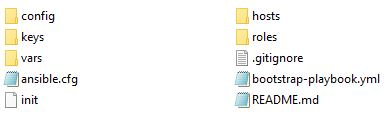
\includegraphics[width=.6\linewidth]{figures/deploy.JPG}}
\caption{Ansible Honeypot Administration Directory}
\end{figure}

\begin{figure}[H]
\frame{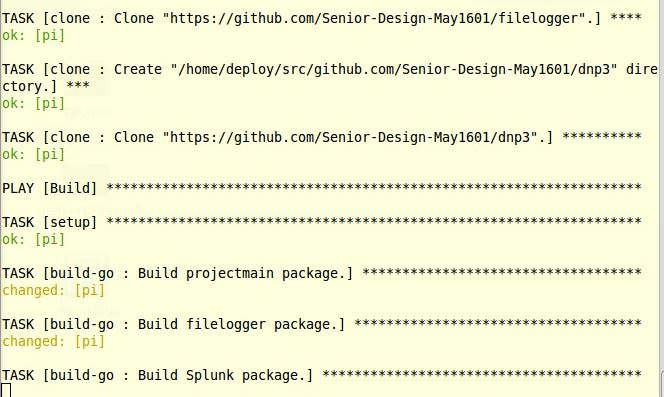
\includegraphics[width=.6\linewidth]{figures/deploy2.JPG}}
\caption{Ansible Honeypot Administration Directory}
%\movie{autostart}{}{figures/out.ogv}
\end{figure}

\end{columns}

\end{frame}

% Slide 13
\begin{frame}
\frametitle{Change Me}

% TODO

\end{frame}

% Slide 14
\begin{frame}
\frametitle{Change Me}

% TODO

\end{frame}

% Slide 15
\begin{frame}
\Huge{\centerline{Questions}}
\end{frame}


\end{document} 
